\documentclass[11pt]{amsart}

\usepackage{amsmath}
\usepackage{amssymb}
\usepackage{tikz}
\usepackage{fp}  % Prevents issues with arithmetic overflow.
\usepackage{pgfplots}
\usepackage{xcolor}
\usepackage[hidelinks]{hyperref}
\usepackage[section]{placeins}  % Prevents figure placement outside of section.
\usetikzlibrary{arrows, fixedpointarithmetic}

\newcommand{\shaft}{\mathrm{shaft}}
\newcommand{\kiteshaft}{\mathrm{kite-shaft}}
\newcommand{\ground}{\mathrm{ground}}
\newcommand{\tether}{\mathrm{tether}}
\newcommand{\bus}{\mathrm{bus}}

\definecolor{matlab1}{rgb}{0, 0.4470, 0.7410}
\definecolor{matlab2}{rgb}{0.8500, 0.3250, 0.0980}
\definecolor{matlab3}{rgb}{0.9290, 0.6940, 0.1250}
\definecolor{matlab4}{rgb}{0.4940, 0.1840, 0.5560}
\definecolor{matlab5}{rgb}{0.4660, 0.6740, 0.1880}
\definecolor{matlab6}{rgb}{0.3010, 0.7450, 0.9330}
\definecolor{matlab7}{rgb}{0.6350, 0.0780, 0.1840}

\title{Motor basics}
\author{Makani Technologies LLC}

\begin{document}
\maketitle

\section{Basic three-phase motor equations}

The basic equations that describe a three-phase motor circuit are
%
\begin{eqnarray}
  \label{eqn:motor_abc}
  v_a &=& R_s i_a + \frac{d\lambda_a}{dt} \\
  v_b &=& R_s i_b + \frac{d\lambda_b}{dt} \\
  v_c &=& R_s i_c + \frac{d\lambda_c}{dt}
\end{eqnarray}
%
where $v_i$ and $i_i$ are the individual phase voltages and currents
and $R_s$ is the single phase stator resistance.  The flux linkages,
$\lambda_i$, are defined such that their derivative is the induced
voltage, and they include both the effects from the self-inductance of
the motor coils as well as the back EMF induced by the permanent
magnets.


\section{Park transformation}

The Park transformation is an \textit{amplitude invariant} coordinate
transformation\footnote{There is a power invariant form of this
  coordinate transformation, which is an orthogonal rotation in a
  vector space spanned by orthogonal $a$, $b$, and $c$ axes about the
  $[1,1,1]^T$ vector.}  to a frame that rotates with the rotor (see
Fig. \ref{fig:dq0}).  Because it is amplitude invariant, the maximum
phase voltage and current remain the same; however, the naive torques
and powers calculations must be scaled by a factor of 3/2.

\begin{figure}[!htb]
  \begin{center}
    \begin{tikzpicture}
      \begin{scope}[scale=4]
        % Draw a, b, c axes.
        \draw [dashed, arrows={-latex}] (0, 0) -- (1, 0) node[below] {$a$};
        \draw [dashed, arrows={-latex}] (0, 0) -- ({-1/2}, {sqrt(3)/2}) node[above] {$b$};
        \draw [dashed, arrows={-latex}] (0, 0) -- ({-1/2}, {-sqrt(3)/2}) node[below] {$c$};

        \begin{scope}[rotate=45]
          % Draw d, q axes.
          \draw [arrows={-latex}] (0, 0) -- (1, 0) node[below] {$d$};
          \draw [arrows={-latex}] (0, 0) -- (0, 1) node[above] {$q$};

          % Draw magnet.
          \draw (0, -0.1) rectangle (0.25, 0.1) node[pos=0.5, rotate=-45] {N};
          \draw (-0.25, -0.1) rectangle (0, 0.1) node[pos=0.5, rotate=-45] {S};
        \end{scope}

        % Draw omega * t.
        \draw [arrows={-latex}] (0.4, 0) arc (0:45:0.4);
        \path (0.4, 0) arc (0:25.5:0.4) node[right] {$\omega_e t$};
      \end{scope}
    \end{tikzpicture}
  \end{center}
  \caption{\label{fig:dq0}Representation of the Park transformation.}
\end{figure}

The transformation is defined by
%
\begin{equation}
  \label{eqn:park}
  \begin{bmatrix}
    f_d \\
    f_q \\
    f_0 \\
  \end{bmatrix}
  = \frac{2}{3}
  \begin{bmatrix}
    \cos (\theta_e)  & \cos (\theta_e - \frac{2 \pi}{3})  & \cos (\theta_e + \frac{2 \pi}{3}) \\
    -\sin (\theta_e) & -\sin (\theta_e - \frac{2 \pi}{3}) & -\sin (\theta_e + \frac{2 \pi}{3}) \\
    \frac{1}{2}    & \frac{1}{2}                        & \frac{1}{2} \\
  \end{bmatrix}
  \cdot
  \begin{bmatrix}
    f_a \\
    f_b \\
    f_c \\
  \end{bmatrix}
\end{equation}
%
where $\theta_e = \omega_e t = p \theta_m$ is the electrical angle of
rotation, and $f_i$ may either be the phase voltages or currents or
the flux linkages.

Also, note that the Park transformation matrix,
$\mathbf{K}(\theta_e) = \mathbf{K}(\omega_e t)$, is a function of
time, so derivatives of parameters transform as
%
\begin{equation}
  \label{eqn:park_deriv}
  \dot{\vec{f}}_{dq0} = \mathbf{K}(\theta_e) \dot{\vec{f}}_{abc} +
                        \omega_e \frac{d \mathbf{K}(\theta_e)}{d\theta_e} \vec{f}_{abc}
\end{equation}

\section{Circuit equations in dq0 coordinates}

Using the Park transformation (Eq. \ref{eqn:park}) and its derivative
(Eq. \ref{eqn:park_deriv}), it is possible to transform the basic
three-phase motor equations (Eq. \ref{eqn:motor_abc}) into a frame
that rotates with the rotor.  Notably, because of the derivative, the
flux linkages transform as
%
\begin{equation}
  \frac{d}{dt}
  \begin{bmatrix}
    \lambda_d \\
    \lambda_q \\
    \lambda_0 \\
  \end{bmatrix}
  +
  \omega_e
  \begin{bmatrix}
    -\lambda_q \\
    \lambda_d \\
    0 \\
  \end{bmatrix}
  = \mathbf{K}(\theta_e) \cdot \frac{d}{dt}
  \begin{bmatrix}
    \lambda_a \\
    \lambda_b \\
    \lambda_c \\
  \end{bmatrix}
\end{equation}
%
Thus, the basic three-phase motor equations may be rewritten in the
rotating frame as
%
\begin{eqnarray}
  v_d &=& R_s i_d + \frac{d\lambda_d}{dt} - \omega_e \lambda_q \\
  v_q &=& R_s i_q + \frac{d\lambda_q}{dt} + \omega_e \lambda_d
\end{eqnarray}
%
In the rotating frame, the flux linkages may be written in terms of
constant inductances along the $d$- and $q$-axes, $L_d$ and $L_q$, as
well as a component due to the permanent magnets, $\lambda_m$, along
the $d$-axis.
%
\begin{eqnarray}
  \lambda_d &=& L_d i_d + \lambda_m \\
  \lambda_q &=& L_q i_q
\end{eqnarray}
%
Finally, the motor dynamics may be written in matrix form as
%
\begin{equation}
  \frac{d}{dt}
  \begin{bmatrix}
    i_d \\
    i_q \\
  \end{bmatrix}
  =
  \begin{bmatrix}
    -R_s / L_d          & \omega_e L_q / L_d \\
    -\omega_e L_d / L_q & -R_s / L_q \\
  \end{bmatrix}
  \cdot
  \begin{bmatrix}
    i_d \\
    i_q \\
  \end{bmatrix}
  +
  \begin{bmatrix}
    1/L_d & 0 \\
    0     & 1/L_q \\
  \end{bmatrix}
  \cdot
  \begin{bmatrix}
    v_d \\
    v_q - \omega_e \lambda_m \\
  \end{bmatrix}
\end{equation}

The steady-state form of these equations,
%
\begin{equation}
  \label{eqn:voltage_limit}
  \begin{bmatrix}
    v_d \\
    v_q \\
  \end{bmatrix}
  =
  \begin{bmatrix}
    R_s          & -\omega_e L_q \\
    \omega_e L_d & R_s \\
  \end{bmatrix}
  \cdot
  \begin{bmatrix}
    i_d \\
    i_q \\
  \end{bmatrix}
  +
  \begin{bmatrix}
    0 \\
    \omega_e \lambda_m \\
  \end{bmatrix}
\end{equation}
%
define a family of ellipses in the phase current plane.  The ellipse
defined by the maximum single phase voltage,
$|v_{dq}| < m \cdot v_{\bus} / \sqrt{3}$, where $m$ is the maximum
modulation index, defines the accesible region of the phase current
plane for a given $\omega_e$.  The center of this voltage-limit
ellipse is given by the short-circuit current:
%
\begin{equation}
  \vec{i}_{sc} =
  \frac{-\omega_e \lambda_m}{R_s^2 + \omega_e^2 L_d L_q}
  \begin{bmatrix}
    \omega_e L_q \\
    R_s
  \end{bmatrix}
\end{equation}
%
Equation \ref{eqn:voltage_limit} may be grossly simplied by assuming,
$L_d = L_q$ (i.e. non-salient motor), and $\omega_e L \gg R_s$.
%
\begin{equation}
  \frac{1}{\omega_e L}
  \begin{bmatrix}
    v_d \\
    v_q \\
  \end{bmatrix}
  =
  \begin{bmatrix}
    0 & -1 \\
    1 & 0 \\
  \end{bmatrix}
  \cdot
  \begin{bmatrix}
    i_d \\
    i_q \\
  \end{bmatrix}
  +
  \begin{bmatrix}
    0 \\
    \lambda_m / L \\
  \end{bmatrix}
\end{equation}
%
In this limit, the relationship between the phase voltage and current
is clear.  The voltage limit circle is centered at
$\vec{i}_{dq} = [-\lambda_m / L, 0]^T$ and has radius
$v_{\max} / \omega_e L$.  The phase voltage axes are rotated
$-\frac{\pi}{2}$ rad from the phase current axes (see
Fig. \ref{fig:voltage_limit}).

\begin{figure}[!htb]
  \begin{center}
    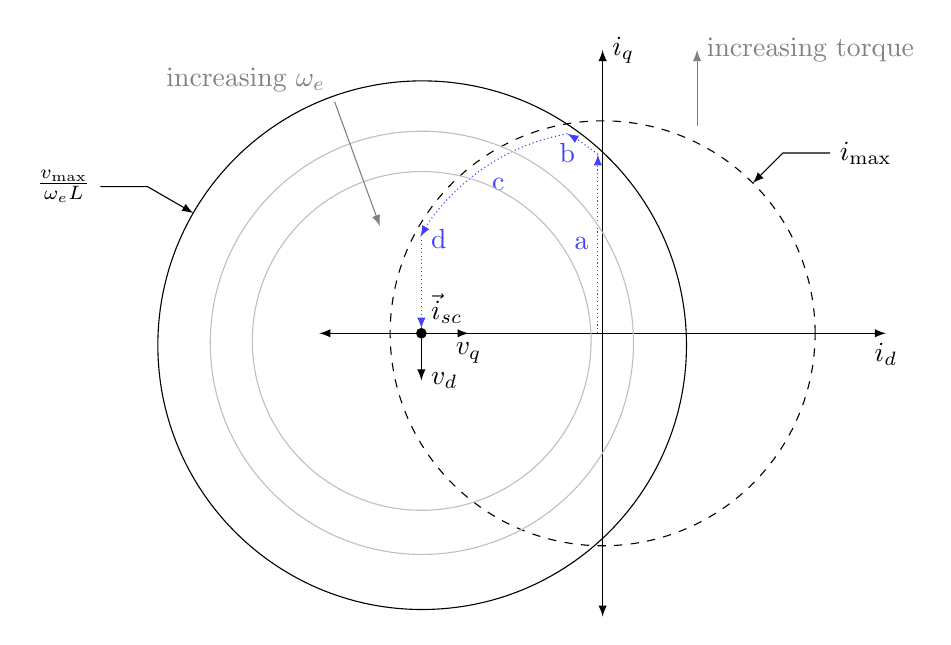
\begin{tikzpicture}[fixed point arithmetic]
      \begin{scope}[scale=0.012]
        \def\Rs{0.103};
        \def\L{0.868e-3};
        \def\lambdam{0.1666};
        \def\Npp{15};
        \def\imax{225};  % [A]
        \def\axislen{300};

        \def\omegam{100};
        \def\omegae{(\omegam * \Npp)};
        \def\znorm{(\Rs * \Rs + \L * \omegae * \L * \omegae)};
        \def\idcenter{(-\omegae * \omegae * \L * \lambdam / \znorm)};
        \def\iqcenter{(-\Rs * \omegae * \lambdam / \znorm)};
        \def\vdqmax{(850.0 / sqrt(3) * 0.95 * 0.94)};
        \def\iradius{(\vdqmax / sqrt(\znorm))};
        \def\iqfw{sqrt(\iradius * \iradius - \idcenter * \idcenter)};
        \def\idsc{(-\lambdam / \L)};

        % Draw axes.
        \draw [arrows={latex-latex}] (-\axislen, 0) -- (\axislen, 0)
              node[below] {$i_d$};
        \draw [arrows={latex-latex}] (0, -\axislen) -- (0, \axislen)
              node[right] {$i_q$};

        % Draw phase current magnitude limit.
        \draw [dashed] (0, 0) circle (\imax);
        \draw [arrows={-latex}] ({1.2 * \imax * cos(45) + 50},
                                 {1.2 * \imax * sin(45)})
                                node[right] {$i_{\max}$} --
                                ({1.2 * \imax * cos(45)},
                                 {1.2 * \imax * sin(45)}) --
                                ({\imax * cos(45)},
                                 {\imax * sin(45)});

        % Draw phase voltage axes.
        \draw [arrows={-latex}] ({\idsc}, 0) -- ({\idsc + 50}, 0) node[below] {$v_q$};
        \draw [arrows={-latex}] ({\idsc}, 0) -- ({\idsc}, -50) node[right] {$v_d$};
        \draw [fill] ({\idsc}, 0) circle (5) node[above right] {$\vec{i}_{sc}$};
        % $(-\frac{\lambda_m}{L}, 0)$};

        % Draw voltage limit circles.
        \def\omegam{120};
        \draw ({\idcenter}, {\iqcenter}) circle ({\iradius});
        \draw [arrows={-latex}] ({1.2 * \iradius * cos(150) - 50 + \idcenter},
                                 {1.2 * \iradius * sin(150) + \iqcenter})
                                node[left] {$\frac{v_{\max}}{\omega_e L}$} --
                                ({1.2 * \iradius * cos(150) + \idcenter},
                                 {1.2 * \iradius * sin(150) + \iqcenter}) --
                                ({\iradius * cos(150) + \idcenter},
                                 {\iradius * sin(150) + \iqcenter});

        % Draw increasing speed path.
        \def\nudge{5};
        \draw [blue!75, densely dotted, arrows={-latex}]
              (-\nudge, 0) -- (-\nudge, {\iqfw - 3*\nudge})
              node [midway, left] {a};
        \draw [blue!75, densely dotted, arrows={-latex}]
              (-\nudge, {\iqfw - 3*\nudge})
              arc
              ({atan2(\iqfw, -\idcenter) + 5}:{atan2(\iqfw, -\idcenter) + 13}:{\iradius})
              node [below] {b}
              coordinate (end);
        \draw [blue!75, densely dotted, arrows={-latex}] (end) arc (100:125:\imax)
              node [below right] {c} arc (125:150:\imax);
        \draw [blue!75, densely dotted, arrows={latex-}] ({\idsc}, \nudge) -- ({\idsc}, 100)
              node [right] {d};

        % Draw higher speed voltage limit circles.
        \def\omegam{150};
        \draw [lightgray] ({\idcenter}, {\iqcenter}) circle ({\iradius});

        \def\omegam{187.5};
        \draw [lightgray] ({\idcenter}, {\iqcenter}) circle ({\iradius});

        %
        \draw [gray, arrows={-latex}]
              ({\idcenter + (\iradius + 90) * cos(110)}, {\iqcenter + (\iradius + 90) * sin(110)})
              node [gray, above left] {increasing $\omega_e$} --
              ({\idcenter + (\iradius - 50) * cos(110)}, {\iqcenter + (\iradius - 50) * sin(110)});

        \draw [gray, arrows={-latex}] (100, 220) -- (100, 300) node [right] {increasing torque};
      \end{scope}
    \end{tikzpicture}
  \end{center}
  \caption{\label{fig:voltage_limit}Phase voltage limits in the phase
    current plane for a non-salient motor in the limit of low stator
    resistance.  The solid circle is the phase voltage limit, whose
    radius decreases as the rotor speed increases.  The dashed circle
    describes the phase current limit, which is determined by gate
    heating.  The blue line shows a typical path for increasing rotor
    speed and power: a) the torque increases, b) flux weakening is
    used to further increase the torque, c) the phase current limit is
    hit but the motor speed is still increasing, and d) the motor is
    in the constant power regime.}
\end{figure}

The equation for torque in $dq0$-coordinates is
%
\begin{eqnarray}
  \tau_e &=& \frac{3}{2} p (\lambda_d i_q - \lambda_q i_d) \\
         &=& \frac{3}{2} p \lambda_m i_q + \frac{3}{2} p (L_d - L_q) i_q i_d \\
         &\approx& \frac{3}{2} p \lambda_m i_q
\end{eqnarray}
%
where $p$ is the number of pole pairs.  The equation for power is
%
\begin{equation}
  P_e = \frac{3}{2} (v_d i_d + v_q i_q)
\end{equation}
%
which under steady-state conditions is
%
\begin{equation}
  P_e = \frac{3}{2}
  \left(
    R_s (i_d^2 + i_q^2) + \omega_e (L_d - L_q) i_q i_d + \omega_e \lambda_m i_q
  \right)
\end{equation}


\begin{table}
  \begin{tabular}{lllll}
    \hline
    \hline
    Parameter                    & Symbol      & Value   &         & Units \\
                                 &             & Protean & Yasa    & \\
    \hline
    Number of pole pairs         & $p$         & 32      & 15      & \# \\
    d-axis inductance            & $L_d$       & 165     & 1000    & $\mu$H \\
    q-axis inductance            & $L_q$       & 165     & 1000    & $\mu$H \\
    Stator resistance            & $R_s$       & 0.041   & 0.103   & $\Omega$ \\
    Permanet magnet flux linkage & $\lambda_m$ & 0.06203 & 0.16667 & N$\cdot$m/A \\
                                 &             &         &         & or V$\cdot$s/rad \\
    \hline
    \hline
  \end{tabular}
  \caption{Motor parameters\protect\footnotemark.}
\end{table}
%
\footnotetext{See
       {\texttt{config/m600/power\_sys\_sim.py}} and \\
       {\texttt{avionics/motor/firmware/params.c}}
}

\section{Space vector pulse width modulation}

The phase voltage vector is controlled using a space vector pulse
width modulation scheme \cite{broek} (see Fig. \ref{fig:svpwm}).

\begin{figure}[ht]
  \begin{center}
    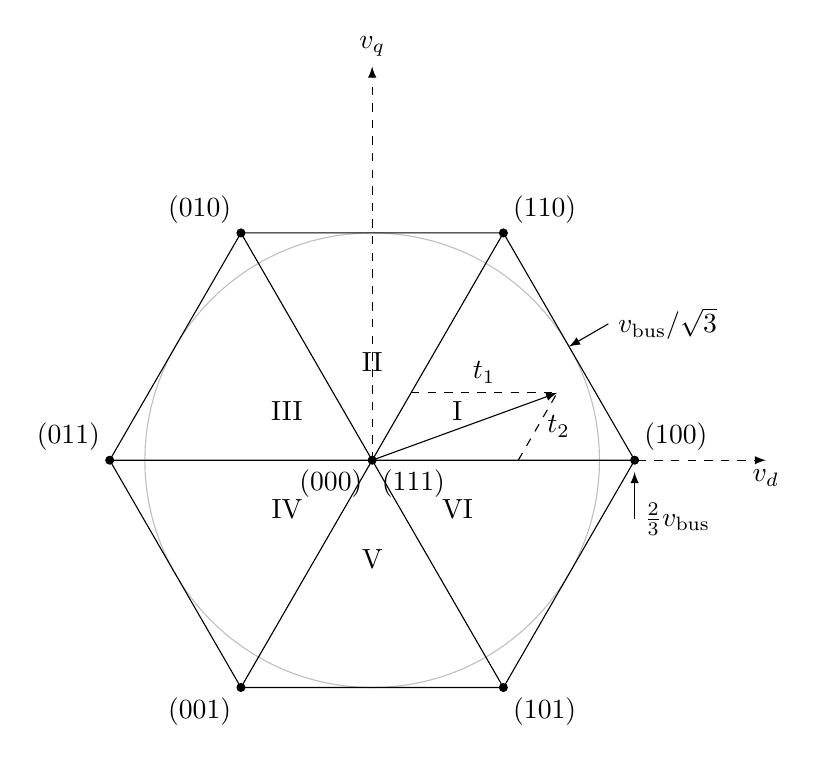
\begin{tikzpicture}
      \begin{scope}[scale=5]
        % Draw d, q axes.
        \draw [dashed, arrows={-latex}] (0, 0) -- (1, 0) node[below] {$v_d$};
        \draw [dashed, arrows={-latex}] (0, 0) -- (0, 1) node[above] {$v_q$};

        % Draw circle.
        \draw [lightgray] (0, 0) circle ({1/sqrt(3)});
        \draw [arrows={latex-}]
              ({1/sqrt(3) * cos(30)}, {1/sqrt(3) * sin(30)}) --
              ({1.2/sqrt(3) * cos(30)}, {1.2/sqrt(3) * sin(30)})
              node [right] {$v_{\bus} / \sqrt{3}$};

        % Draw hexagon.
        \draw (2/3, 0) -- (1/3, {1/sqrt(3)}) -- (-1/3, {1/sqrt(3)}) --
              (-2/3, 0) -- (-1/3, {-1/sqrt(3)}) -- (1/3, {-1/sqrt(3)}) --
              (2/3, 0);
        \draw [fill] (0, 0) -- (2/3, 0) circle (0.01)
              node [above right] {(100)};
        \draw [arrows={latex-}] (2/3, -0.03) -- (2/3, -0.15)
              node [right] {$\frac{2}{3} v_{\bus}$};
        \draw [fill] (0, 0) -- (1/3, {1/sqrt(3)}) circle (0.01)
              node [above right] {(110)};
        \draw [fill] (0, 0) -- (-1/3, {1/sqrt(3)}) circle (0.01)
              node [above left] {(010)};
        \draw [fill] (0, 0) -- (-2/3, 0) circle (0.01)
              node [above left] {(011)};
        \draw [fill] (0, 0) -- (-1/3, {-1/sqrt(3)}) circle (0.01)
              node [below left] {(001)};
        \draw [fill] (0, 0) -- (1/3, {-1/sqrt(3)}) circle (0.01)
              node [below right] {(101)};

        \draw [fill] (0, 0) circle (0.01)
              node [below left] {(000)} node [below right] {(111)};

        \path (0, 0) -- ({0.25 * cos(30)}, {0.25 * sin(30)}) node {I};
        \path (0, 0) -- ({0.25 * cos(90)}, {0.25 * sin(90)}) node {II};
        \path (0, 0) -- ({0.25 * cos(150)}, {0.25 * sin(150)}) node {III};
        \path (0, 0) -- ({0.25 * cos(210)}, {0.25 * sin(210)}) node {IV};
        \path (0, 0) -- ({0.25 * cos(270)}, {0.25 * sin(270)}) node {V};
        \path (0, 0) -- ({0.25 * cos(330)}, {0.25 * sin(330)}) node {VI};

        % Draw PWM vector.
        \draw [arrows={-latex}] (0, 0) -- ({0.5 * cos(20)}, {0.5 * sin(20)});
        \draw [dashed] ({0.5 * sin(20) * tan(30)}, {0.5 * sin(20)}) --
                       ({0.5 * cos(20)}, {0.5 * sin(20)}) node [midway, above] {$t_1$};
        \draw [dashed] ({0.5 * (cos(20) - sin(20) * tan(30))}, 0) --
                       ({0.5 * cos(20)}, {0.5 * sin(20)}) node [midway, right] {$t_2$};

      \end{scope}
    \end{tikzpicture}
  \end{center}
  \caption{\label{fig:svpwm}Space vector pulse width modulation.  The
    six corners of the hexagon represent six of the on-off states of
    the three switches on one side of the H-bridge.}
\end{figure}


\section{Motor limits}

\subsection{Source power limit}

The total shaft power of the motors is limited by the maximum ground
power as well as the efficiency losses from the tether, inverters, and
motors.  This constraint is expressed as:
%
\begin{equation}
  \sum_i P_{\shaft, i} < \eta_{\kiteshaft}
  \left( 1 - \frac{P_{\ground} R_{\tether}}{V_{\ground}^2} \right) P_{\ground}
\end{equation}

\begin{table}
  \begin{tabular}{llll}
    \hline
    \hline
    Parameter & Symbol & Value & Units \\
    \hline
    Kite-bus-to-shaft efficiency    & $\eta_{\kiteshaft}$ & 0.88 & \# \\
    Ground power (SatCon I)         & $P_{\ground}$       & 660  & kW \\
    Ground power (SatCon II)        & $P_{\ground}$       & 1000 & kW \\
    Tether resistance               & $R_{\tether}$       & 0.8  & $\Omega$ \\
    Ground voltage                  & $V_{\ground}$       & 3400 & V \\
    Phase current limit             & $i_{dq,\max}$       & 225  & A \\
    Flux weakening modulation limit & $m_{\mathrm{fw}}$   & 0.95 & \# \\
    Gate hold time modulation limit & $m_{\mathrm{gate}}$ & 0.94 & \# \\
    \hline
    \hline
  \end{tabular}
  \caption{Power source and motor limitation parameters\protect\footnotemark.}
\end{table}

\footnotetext{See {\texttt{config/m600/power\_sys.py}}}

\subsection{Phase current limit}

The motor controllers enforce a phase current magnitude limit to
control the maximum temperature that the SiC modules can reach\footnote{See
       {\texttt{go/makanimotorthermallimits}}}.
%
\begin{equation}
  i_d^2 + i_q^2 < i_{dq,\max}^2
\end{equation}
%
This is the dashed line shown in Fig. \ref{fig:voltage_limit}.  Before
flux weakening was implemented, this constraint was called a ``torque
limit'' as $\tau \propto i_q$.  However, with flux weakening and
consequently non-zero $i_d$ values, it is more accurately refered to
as a phase current limit.  Currently, $i_{dq,\max} = 225$
A\footnote{See
  {\texttt{config/m600/power\_sys\_sim.py}} and \\
  {\texttt{avionics/motor/firmware/foc.c}}}; though it
could potentially be raised in the future.

\subsection{Motor power limit}

The maximum power the motor can deliver occurs when the current
command is at the top of the voltage limit circle.  Here, even as the
motor speed increases and the voltage-limit circle shrinks, the power
remains constant because the radius of the circle is inversely
proportional to the motor speed.  An approximate equation for the
maximum power is
%
\begin{equation}
  P_{\max} \approx \frac{3}{2} \frac{\lambda_m}{L_q} m \frac{v_{\bus}}{\sqrt{3}}
\end{equation}
%
where $m$ is the maximum modulation index, including the gate hold
times.  Currently, $m = 0.95 \times 0.94$ where the first term is the
maximum modulation allowed by flux weakening and the second term is
the maximum duty cycle allowed by the gate hold times.

Because parameters such as $\lambda_m$ change significantly at high
torques, it is better to measure the maximum power empirically.  The
maximum motor shaft power was measured to be
$P_{\shaft,\max} \approx 108$ kW.

A more exact equation for the maximum power is
%
\begin{equation}
  P_{\max} =
  \frac{3}{2} \lambda_m \omega_e
  \left(
    \frac{m \cdot v_{\bus} / \sqrt{3}}{\sqrt{R_s^2 + \omega_e^2 L_q^2}} -
    \frac{R_s \omega_e \lambda_m}{R_s^2 + \omega_e^2 L_d L_q}
  \right)
\end{equation}

\section{Base speed}

The constant torque section of the speed-power curve ends when the
voltage limit circle intersects the $i_q$ axis at the maximum phase
current.
%
\begin{equation}
  \omega_{m, r_1} = \frac{v_{\max}}{p L \sqrt{i_{\max}^2 + i_{d,sc}^2}}
\end{equation}
%
The constant power section of the speed-power curve begins when the
top of the voltage limit circle intersects the maximum phase current
limit circle.
%
\begin{equation}
  \omega_{m, r_2} = \frac{v_{\max}}{p L \sqrt{i_{\max}^2 - i_{d,sc}^2}}
\end{equation}

\begin{thebibliography}{1}
\bibitem{broek} H. Broeck et. al. ``Analysis and realization of a
  pulsewidth modulator based on space vectors.'' IEEE
  Trans. Industry. App., \textbf{24}, 1 (1988).
\end{thebibliography}

\end{document}
